\documentclass[]{scrartcl}
\usepackage[utf8]{inputenc}
\usepackage{graphicx}
\usepackage{amsmath}
\usepackage{float}

\title{Modellierung dynamischer Systeme  \\ Entwurf zur Bearbeitung der Praktikumsaufgabe 3}

\author{Maria Lüdemann und Birger Kamp}

\begin{document}

\maketitle

\begin{abstract}

\end{abstract}

\section{Schiefer Flipper}
Im Vorlauf der Praktikumsaufgabe 3 haben wir uns dafür entschieden den schiefen Flipper zu simulieren.

Dafür soll die Bewegung einer Kugel auf einer geneigten Ebene simuliert werden. Die Ebene ist von drei Wänden begrenzt und hat in der Mitte ein zylindrisches Hindernis. Das Abprallen der Kugel von den Wänden und dem Hindernis verändert die Richtung ihrer Bewegung, dabei wird auch ihre Beschleunigung und somit Geschwindigkeit simuliert.


\begin{figure}[H]
\centering
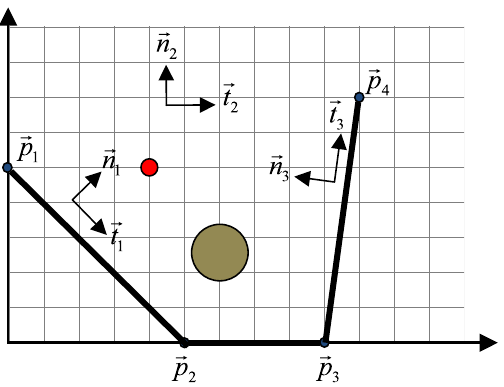
\includegraphics[width=0.8\linewidth]{./skizze_schieferFlipper}
\caption{Skizze zum schiefen Flipper}
\label{fig:1_skizze_schieferFlipper}
\end{figure}


\subsection{Gegebene Formeln und Konstanten}
Die begrenzenden Wände, durch Vektoren dargestellt definieren sich als:
\begin{align}
\vec{p_1} = (0,5)^T \ 
\vec{p_2} = (5,0)^T \ 
\vec{p_3} = (9,0)^T \ 
\vec{p_4} = (10,7)^T
\end{align}

Die Position und der Umfang des zylindrischen Hindernisses entsprechen:
\begin{align}
\vec{p_Z} = (6,2.5)^T \ 
RHnd = 0.8
\end{align}

Startposition der Kugel
\begin{align}
\vec{xa}_{0} = (4,5)^T
\end{align}

Startgeschwindigkeit der Kugel
\begin{align}
\vec{v1}_{0} = (0,0)^T
\end{align}

Radius der Kugel
\begin{align}
R = 0.25
\end{align}


\subsection{Simulationsrandbedingungen}
Die Variablen Konstanten und Parameter für diese Aufgabe sind stark vorgegeben und werden dem der Aufgabenstellung beigefügten Bild entnommen. Dieses Bild ist untenstehend gezeigt. Dabei handelt es sich bei $RHnd$ um den oben definierten Radius des Zylinderhindernisses. $R$ ist der oben definierte Radius der Kugel und $Hnd$ der Ort, also Positionsvektor des Zylinderhindernisses wie oben als $\vec{p_Z}$ bestimmt.


\subsection{Funktionen}
Um das System zu simulieren wurden einige Funktionen vorgegeben die entworfen werden müssen. 

\subsubsection{Init}
Die Funkion Init die die folgenden benötigten Größen initialisiert:
\begin{itemize}
\item Wandeckpunkte ($\vec{p_1}, \vec{p_2}, \vec{p_3}, \vec{p_4}$)und Hindernispositionen $\vec{p_Z}$
\item Zustandsgrößen
\item die Wand-Tangential und Normalvektoren,
\item Startposition $\vec{xa}_{0}$ und Startgeschwindigkeit $\vec{v1}_{0}$ der Kugel
\end{itemize}

\subsubsection{Acceleration}
Die Funktion $Acc()$ soll die Beschleunigung $a$ der Kugel berechnen.

\subsubsection{Wand..Kontakt}
Für jede der drei Wände muss es eine Funktion geben die den Kontakt zwischen der Wand und der Kugel feststellt. Dafür wird ein $true$ zurück gegeben wenn die Kugel in der Vorwärtsbewegung die Wand berührt.

\subsubsection{Wand..Reflexion}
Für jede der drei Wände muss eine Funktion geschrieben werden die wenn die dazugehörige Wand..Kontakt Funktion $true$ liefert die Reflexion der Kugel von der Wand realisiert.

\subsubsection{Hindernis Kontakt}
Es wird eine Funktion benötigt die den Kontakt mit dem Hindernis berechnet und genau wie $Wand..Kontakt$ ein $true$ zurück gibt wenn die Kugel das Hindernis in der Vorwärtsbewegung berührt.

\subsubsection{Hindernis Reflexion} 
Um die Reflexion der Kugel am Hindernis zu simulieren muss eine Funktion $HndRefl()$ geschrieben werden die die Reflexion der Kugel berechnet wenn die dazugehörige $HndKontakt$ ein $true$ liefert.

\subsubsection{Zustand}
Der Zustand selber soll in der $during$-Sektion die Differentialgleichungen und die Übergabe an die Ausgangsgröße abhandeln.

\subsubsection{Simulation}
Die Simulation soll mit dem Programm $Table.wrl$ dargestellt und visualisiert werden.


\subsection{Versuchsdurchführung}

Die Simulation soll mit den Einstellungen $Non-adaptive$ für den $Zero-crossing algorithm$  gestartet werden. Dafür gibt es eine vorgegeben Einstellung in der Aufgabenstellung für die VR-Sink. Das folgende Bild ist aus der Aufgabenstellung übernommen und zeigt die nötigen Einstellungen.


\begin{figure}[H]
\centering
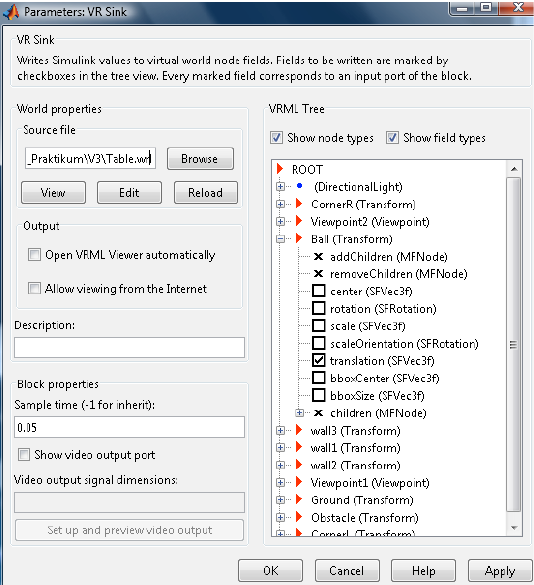
\includegraphics[width=0.8\linewidth]{./einstellungen_schieferFlipper}
\caption{Einstellung für die Versuchsdurchführung}
\label{fig:2_einstellungen_schieferFlipper}
\end{figure}
 
\end{document}
